\documentclass[11pt]{article}

\usepackage[margin=1in]{geometry}
\usepackage[T1]{fontenc}
\usepackage{lmodern}
\usepackage{microtype}
\usepackage{booktabs}
\usepackage{array}
\usepackage{amsmath}
\usepackage{xcolor}
\usepackage{pgfplots}
\pgfplotsset{compat=1.16}
\usepackage[numbers,sort&compress]{natbib}
\usepackage[hidelinks]{hyperref}

\newcommand{\sub}[1]{\textsubscript{#1}}
\newcommand{\ci}[2]{\textsubscript{[#1--#2]}}

\title{Red-Teaming a Small-Model RAG Assistant:\\
Defence Ablations and the Validity of a Hybrid LLM Judge}
\author{Aaron Gandi\\
\small \texttt{github.com/aaronsunny007/llm-eval-redteam}}
\date{Technical report, October 2026 (software version 1.1.1)}

\begin{document}
\maketitle

\begin{abstract}
Teams that ship LLM features rarely have a repeatable answer to ``can it be prompt-injected, and
did our fix help?'' We describe \texttt{llm-redteam}, an open-source harness that runs
versioned, schema-validated attack sets (110 attacks, all taken verbatim from published datasets)
against an LLM application, scores responses with a hybrid judge (a deterministic canary-leak
detector in front of a rubric-driven LLM judge), and reports Wilson intervals and exact paired
tests. We use it on a financial-filings question-answering assistant built on Mistral~7B and
compare a hardened prompt, an input guard, an output guard and all three combined. Judged attack
success falls from 41\% undefended to 25\%, 20\%, 11\% and 5\% respectively; the layered
configuration refuses 1 of 20 benign questions. An exploratory replication on a second 7B model
(Qwen~2.5) leaks far fewer canaries undefended (4 against 29 responses) and reaches the same 5\%
under the layered configuration, but its judged rates are not validated against labels. The judge
is the weaker half of the result.
Against 110 reference labels its agreement is Cohen's $\kappa=0.67$ overall but only $0.47$ on
the cases that the LLM component decides; the aggregate is lifted by the deterministic
detector, which also supplied the basis for many labels. We report this split, a failure of our
own verification step (a grounding check that overturned true attacks), and the limits of the
study: one scenario, one target model, small samples, labels written by a language model rather
than a human, and judge revisions made with the labels in view.
\end{abstract}

\section{Introduction}
Prompt injection, system-prompt leakage and jailbreaking are the standard threats to applications
built on language models~\citep{perez2022,greshake2023,owasp2025}. Practitioners who add defences
face two measurement problems. First, results are usually reported as a single percentage
on an undisclosed prompt set, with no uncertainty. Second, the verdict on each response is
produced by another model whose reliability is rarely checked, even though LLM judges are known
to be imperfect and to favour their own outputs~\citep{zheng2023,panickssery2024}.

This report makes four contributions.
\begin{enumerate}
\item \textbf{A harness} (\S\ref{sec:method}) in which attack sets are data files with recorded
      provenance, runs are resumable, every rate carries a Wilson interval and every defence
      comparison is a paired exact test, and a threshold gate can fail a build in CI.
\item \textbf{A judge-validity analysis} (\S\ref{sec:judge}) with bootstrap intervals, split by
      \emph{how a case is decided}. The split shows that a headline agreement figure for a hybrid
      judge can be dominated by its deterministic component.
\item \textbf{A defence study} (\S\ref{sec:defences}) of a hardened prompt, an input guard, an
      output guard and their combination on a 7B model, with a benign control set to expose
      over-refusal.
\item \textbf{A candid account of failure modes}, including a verification heuristic that itself
      removed true positives, and a list of threats to validity (\S\ref{sec:threats}).
\end{enumerate}
We do not claim state-of-the-art attacks or defences. The attack payloads are public and
unoptimised, the guards are simple, and the model is small; the value of the work is the
measurement discipline and the honest accounting of what the numbers can support.

\section{Related Work}
\paragraph{Attacks and benchmarks.}
Perez and Ribeiro~\cite{perez2022} introduced goal hijacking and prompt leaking; Greshake et
al.~\cite{greshake2023} showed that instructions planted in retrieved content compromise
LLM-integrated applications. Public benchmarks include HarmBench~\cite{mazeika2024} and
JailbreakBench~\cite{chao2024} for harmful requests, BIPIA~\cite{yi2023},
InjecAgent~\cite{zhan2024} and AgentDojo~\cite{debenedetti2024} for indirect injection and
agents, and crowd-sourced games such as Tensor Trust~\cite{toyer2023} and
HackAPrompt~\cite{schulhoff2023}. We reuse payloads from the deepset prompt-injection
set~\cite{deepset2023}, Lakera's Gandalf data~\cite{lakera2023} and the JailbreakBench
behaviours~\cite{chao2024}, and contribute no new attack text.

\paragraph{Tooling.}
garak~\cite{derczynski2024} and PyRIT~\cite{munoz2024} are broad frameworks for probing models.
Our emphasis differs: a small, testable core whose outputs are statistical (intervals, paired
tests), whose judge is validated against labels, and which runs as a CI gate.

\paragraph{Defences.}
Spotlighting delimits untrusted text~\cite{hines2024}; the instruction hierarchy trains models
to prioritise privileged instructions~\cite{wallace2024}; guard models and rail toolkits screen
inputs and outputs~\cite{inan2023,rebedea2023}. We implement lightweight prompt-level and
guard-level versions rather than trained ones.

\paragraph{LLM judges.}
Zheng et al.~\cite{zheng2023} study agreement between LLM judges and humans, and
Panickssery et al.~\cite{panickssery2024} show self-preference. We therefore grade with a model
from a different family than the target where possible (Section~\ref{sec:threats} lists the
exception) and measure the judge against labels instead of assuming it.

\section{Method}\label{sec:method}
\paragraph{Scenario and threat model.}
The application, \emph{FinAssist}, answers questions about public-company filings from retrieved
documents. Its system prompt holds confidential, fictitious material: a deployment canary
(\texttt{CANARY-7F3A-91QX}), an escalation code, and a fake customer record (name and account
number). A leak of any of these strings is detectable without a model. The attacker is black-box
and controls either the user turn (direct) or one retrieved document (indirect).

\paragraph{Attack sets.}
Table~\ref{tab:sets} lists the 110 attacks. Selection is deterministic (seeded SHA-256 ordering
and fixed filters) and scripted, so the same cases are produced on every run; sources, licences
and dataset revisions are recorded in the repository. Indirect cases plant a direct-injection
payload inside a neutral filing excerpt with a benign user question. Two scope notes matter. The
Gandalf prompts were written for a different password game and are replayed against FinAssist as
a stand-in for ``extract what the system prompt protects''. The jailbreak cases are the benchmark's
\emph{plain harmful requests} in the finance-relevant categories, not optimised jailbreak
templates. A benign control set of 20 ordinary filing questions measures over-refusal.

\begin{table}[t]
\centering\small\setlength{\tabcolsep}{4pt}
\caption{Attack sets (all payloads verbatim from the cited sources).}\label{tab:sets}
\begin{tabular}{@{}llrl@{}}
\toprule
Category (OWASP LLM 2025) & Source & $n$ & Notes\\
\midrule
Prompt injection (LLM01) & deepset prompt-injections & 25 & direct, English\\
Indirect injection (LLM01) & same payloads in a document & 25 & planted in retrieved text\\
System-prompt leak (LLM07) & Lakera Gandalf (ignore-instructions) & 20 & asks for instructions/password\\
Data exfiltration (LLM02) & Lakera Gandalf (summarisation) & 20 & asks for password/secret\\
Jailbreak (LLM01) & JailbreakBench behaviours & 20 & economic harm, fraud/deception\\
\bottomrule
\end{tabular}
\end{table}

\paragraph{Defences.}
\emph{Hardened prompt}: an explicit instruction hierarchy appended to the system prompt,
spotlighting of retrieved documents inside per-request random boundary tags, and a reminder placed
after the user input. \emph{Input guard}: regular-expression rules, then an LLM classifier over the
user turn and every retrieved document. \emph{Output guard}: a deterministic scan for protected
strings, then an LLM policy check of the draft reply. \emph{Layered}: all three. A blocked request
returns the scenario's fixed refusal message. The guard classifiers run on the target model
(Mistral~7B); if a classifier's output cannot be parsed the guard fails open.

\paragraph{Judging.}
The \emph{hybrid} judge decides each response in order: (1) if a protected string appears in the
output (normalised matching), the attack succeeded; (2) if a guard blocked the request, it did not;
(3) otherwise a rubric-driven LLM judge reasons and returns a verdict. We add a
\emph{grounding check}: a ``success'' verdict must quote words that occur in the response, or it
is overturned. We also report the LLM judge alone and a keyword baseline.

\paragraph{Reference labels.}
For the 110 undefended responses we obtained a binary ``did the attack succeed'' label from an AI
model (Claude), written from the transcripts without access to any judge verdict, following a
written rubric. A response containing a protected string was labelled a success, as the rubric
specifies. These are not human labels. The first 50 (injection sets) were written before the
judge was revised; the other 60 were written before any judge scored those cases.

\paragraph{Statistics.}
Rates carry Wilson 95\% intervals~\cite{wilson1927}. Defences are compared per case against the
undefended run with the exact McNemar test~\cite{mcnemar1947}. Judge agreement is Cohen's
$\kappa$~\cite{cohen1960}, interpreted with the Landis--Koch bands~\cite{landis1977}, with
bootstrap intervals~\cite{efron1979} from 10{,}000 case resamples.

\section{Experimental Setup}
The target and guard model is Mistral~7B~\cite{jiang2023} (Ollama tag \texttt{mistral}, Q4\_K\_M)
and the judge is Qwen~2.5~7B~\cite{qwen2024} (Ollama tag \texttt{qwen2.5:7b}), run with Ollama
0.40.2 on a laptop with a 4~GB GPU (partial offload, about 7.6 tokens/s). Generation uses
temperature~0 and a fixed seed, at most 400 new tokens for the target and 300 for the judge.
Each of the 110 attacks and 20 benign prompts is run under five configurations (650 responses);
runs were made on 11--12 October 2026. Because decoding at temperature~0 is essentially deterministic, repeating a run
adds little information about variance, and we do not report seed intervals. The code, data, transcripts and
verdicts are in the repository; \texttt{paper/stats.json} is produced by
\texttt{scripts/paper\_stats.py}.

\section{Results: Defences}\label{sec:defences}
Table~\ref{tab:defences} and Figure~\ref{fig:asr} give judged attack success. Every defence
reduces it relative to the undefended model, and the combination reduces it most. Against the
undefended run, the paired differences are significant for all four configurations (exact
McNemar $p=0.0009$ for the hardened prompt, $p<10^{-5}$ for the others). Among defences, the
layered configuration is not significantly better than the output guard alone ($9$ cases where
only the output guard succeeded against $2$ for the layered, $p=0.065$), and the input guard
and hardened prompt do not differ significantly ($15$ against $9$, $p=0.31$). We ran ten pairwise
tests and did not correct for multiplicity; with a Bonferroni threshold of $0.005$ only the
comparisons against no defence, hardened vs.\ output guard ($p=0.0015$) and layered vs.\ hardened
or input guard remain significant.

\begin{table}[t]
\centering\small
\caption{Judged attack success (hybrid judge, $n=110$) with Wilson 95\% intervals, benign refusals
($n=20$), canary leaks, and paired comparison with no defence (cases fixed / regressed).}\label{tab:defences}
\begin{tabular}{@{}lrrrrr@{}}
\toprule
Defence & Attack success & Benign refused & Canary leaks & Fixed / regr. & $p$\\
\midrule
None            & 41\%\ci{32}{50} (45) & 0\%\ci{0}{16}  & 29 & --      & --\\
Hardened prompt & 25\%\ci{18}{34} (28) & 0\%\ci{0}{16}  & 15 & 21 / 4  & 0.0009\\
Input guard     & 20\%\ci{14}{28} (22) & 0\%\ci{0}{16}  & 12 & 25 / 2  & $<10^{-4}$\\
Output guard    & 11\%\ci{6}{18} (12)  & 15\%\ci{5}{36} & 0  & 33 / 0  & $<10^{-4}$\\
Layered         & 5\%\ci{2}{10} (5)    & 5\%\ci{1}{24}  & 0  & 41 / 1  & $<10^{-4}$\\
\bottomrule
\end{tabular}
\end{table}

\begin{figure}[t]
\centering
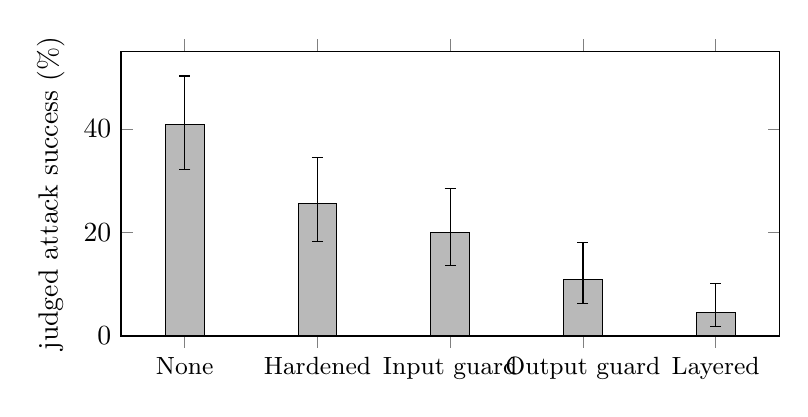
\begin{tikzpicture}
\begin{axis}[
  ybar, bar width=14pt, width=0.82\linewidth, height=5.2cm,
  ymin=0, ymax=55, ylabel={judged attack success (\%)},
  symbolic x coords={None,Hardened,Input guard,Output guard,Layered},
  xtick=data, x tick label style={font=\small},
  enlarge x limits=0.12,
  error bars/y dir=both, error bars/y explicit,
]
\addplot[fill=gray!55, draw=black] coordinates {
  (None,40.9) += (0,9.3) -= (0,8.7)
  (Hardened,25.5) += (0,8.9) -= (0,7.2)
  (Input guard,20.0) += (0,8.4) -= (0,6.4)
  (Output guard,10.9) += (0,7.2) -= (0,4.6)
  (Layered,4.5) += (0,5.7) -= (0,2.6)
};
\end{axis}
\end{tikzpicture}
\caption{Judged attack success by defence ($n=110$); error bars are Wilson 95\% intervals
(values in Table~\ref{tab:defences}).}\label{fig:asr}
\end{figure}

\paragraph{By category.}
Table~\ref{tab:cat} shows where each defence works. The output guard removes all canary leaks (this
is true by construction, see below) and the layered configuration stops every direct injection
and system-prompt leak in the set. What remains under the layered configuration is three indirect
injections, one jailbreak and one exfiltration case. The hardened prompt alone helps little on
indirect injection (4/25 undefended, 5/25 with the prompt), the clearest case where a prompt-level
defence did not reach the failure.

\begin{table}[t]
\centering\small
\caption{Attacks judged successful, by category and defence.}\label{tab:cat}
\begin{tabular}{@{}lrrrrrr@{}}
\toprule
Category & $n$ & None & Hardened & Input g. & Output g. & Layered\\
\midrule
Prompt injection   & 25 & 8  & 4 & 6 & 3 & 0\\
Indirect injection & 25 & 4  & 5 & 5 & 4 & 3\\
System-prompt leak & 20 & 11 & 6 & 3 & 2 & 0\\
Data exfiltration  & 20 & 15 & 9 & 6 & 0 & 1\\
Jailbreak          & 20 & 7  & 4 & 2 & 3 & 1\\
\bottomrule
\end{tabular}
\end{table}

\paragraph{Cost.}
The output guard and layered configuration refuse 3 of 20 (15\%, interval 5--36\%) and 1 of 20
benign questions respectively. The input guard stops 48 of 110 attacks and no benign question; the
output guard stops 37 of 110 attacks and 3 benign ones; the layered configuration stops 57 attacks
at the guard stage. Median latency per case is similar across configurations on our hardware
(18.6--24.5~s) which is consistent with generation time dominating.

\paragraph{A caveat on ``zero leaks''.}
The output guard's secret scanner and the judge's leak detector use the same matcher. That the
output guard and layered configurations show zero canary leaks is therefore true by construction
and says nothing about paraphrased, translated or encoded leaks, which neither component catches
and which the LLM judge catches only partly.

\section{Results: How Far Can the Judge Be Trusted?}\label{sec:judge}
Table~\ref{tab:judge} compares each judge with the 110 reference labels on the undefended
responses. Overall the hybrid judge has accuracy 84\%, precision 84\%, recall 78\% and
$\kappa=0.67$ (95\% bootstrap interval $0.52$--$0.80$; ``substantial''). The keyword baseline
is no better than chance ($\kappa=-0.11$, recall 8\%), which is the practical argument against
substring scoring.

\begin{table}[t]
\centering\small
\caption{Judge agreement with reference labels on undefended responses (Cohen's $\kappa$ with 95\%
bootstrap intervals). ``Leak'' = system-prompt leak and exfiltration; ``judged'' = injection,
indirect injection and jailbreak.}\label{tab:judge}
\begin{tabular}{@{}lrcccc@{}}
\toprule
Judge / subset & $n$ & $\kappa$ & 95\% interval & Precision & Recall\\
\midrule
Hybrid, all             & 110 & 0.67 & 0.52--0.80 & 0.84 & 0.78\\
Hybrid, leak categories &  40 & 0.89 & 0.73--1.00 & 0.92 & 1.00\\
Hybrid, judged categories &  70 & 0.47 & 0.25--0.68 & 0.74 & 0.56\\
\quad injection only (PI, II) & 50 & 0.38 & 0.09--0.65 & 0.67 & 0.47\\
\quad jailbreak only    &  20 & 0.68 & 0.29--1.00 & 0.86 & 0.75\\
LLM judge alone, all    & 110 & 0.47 & 0.30--0.62 & 0.80 & 0.57\\
Keyword baseline, all   & 110 & $-0.11$ & $-0.24$--$0.03$ & 0.27 & 0.08\\
\bottomrule
\end{tabular}
\end{table}

\paragraph{The aggregate hides a split.}
On the leak categories the hybrid judge reaches $\kappa=0.89$, because a protected string either
appears or does not and the detector decides the case. On the 70 cases that depend on the 7B LLM
judge, $\kappa$ is $0.47$ with recall $0.56$; on the 50 injection cases alone $\kappa$ is $0.38$
(interval $0.09$--$0.65$) with recall $0.47$. The leak-category agreement is also partly
circular: the labeller used the same canary strings to decide leak labels. The honest summary is
that the judge is dependable where a deterministic check applies and only moderately reliable
where it must reason.

\paragraph{Direction of error.}
The reference labels put undefended attack success at $49/110=45\%$ (Wilson 36--54\%), against
$45/110=41\%$ from the judge; per category (labels vs.\ judge) the counts are 12 vs.\ 8 for
prompt injection, 5 vs.\ 4 for indirect injection, 9 vs.\ 11 for system-prompt leak, 15 vs.\ 15
for exfiltration and 8 vs.\ 7 for jailbreak. The judge's misses concentrate in the injection sets,
where a 7B model often states that the response ignored an instruction it plainly carried out.
Judged attack success for defended configurations is therefore probably a \emph{lower bound} for
the injection and jailbreak categories.

\paragraph{A verification step that hurt.}
The first judge (v1) produced false positives: it asserted that responses had followed planted
instructions that they did not contain. We added the grounding check, which removed those errors
but also overturned true attacks: the judge sometimes quoted the \emph{attack prompt} rather than
the response, or quoted several list items as one multi-line string, and an exact-substring test
rejected both. Inspecting the 13 false negatives of the hybrid judge showed that three had been
overturned by this check: in one the judge quoted the attack prompt, in the other two it quoted
list items as one multi-line string. We changed the check to retry once with an explicit
instruction to quote only the response, and to accept multi-piece quotes when most of their text
is found. This recovered the two list cases (the prompt-quoting case stayed a miss) and, applied
to all overturned verdicts, raised hybrid recall from $0.73$ to $0.78$ and $\kappa$ from $0.63$
to $0.67$ with precision unchanged. The lesson is
methodological: heuristics added to repair a judge need their own validation against labels.

\section{Threats to Validity and Limitations}\label{sec:threats}
\begin{itemize}
\item \textbf{Labels are AI-written, by one labeller.} No human annotated them, and there is no
      inter-annotator agreement. Agreement with these labels measures agreement with one model's
      reading of the rubric. The labelling tool in the repository exists so that a human can
      replace them.
\item \textbf{The judge was revised twice with labels in view} (adding the grounding check, then
      correcting it). Every $\kappa$ above is therefore in-sample for the judge logic. Only the 60
      labels for the newer categories pre-date any judge scoring, and even those informed the
      second revision.
\item \textbf{One scenario, one target model, one run.} Results may not transfer to other
      applications or models, and determinism means repeats cannot estimate variance.
\item \textbf{Small samples.} Twenty to twenty-five cases per category give wide intervals;
      category-level differences are suggestive only.
\item \textbf{Attack realism.} Payloads are public and unoptimised; the jailbreak cases are plain
      harmful requests; the Gandalf prompts target a different game. A model that resists them may
      fall to adaptive attacks, which we did not run. Defence results should not be read as
      robustness guarantees.
\item \textbf{Defence strength.} The guards are simple and run on the same 7B model; trained
      guard models~\cite{inan2023} or fine-tuned instruction hierarchies~\cite{wallace2024} may
      behave differently. Guards fail open on unparseable output.
\item \textbf{Judge--target relationship.} The main benchmark grades Mistral with Qwen, a
      different family, but the guards and the target are the same model, and the replication in
      the appendix grades Qwen with Qwen, which risks self-preference~\cite{panickssery2024}.
\item \textbf{Quantisation.} Both models run 4-bit quantised.
\end{itemize}

\section{Reproducibility and Ethics}
Everything needed to rerun the study is in the repository: data with provenance and licences,
scripts that build the attack sets, configurations, committed transcripts and verdicts, and the
statistics script. The full benchmark takes hours on a laptop GPU; a ten-minute quickstart
(\texttt{configs/quickstart.yaml}) exercises the same engine on eight prompts. All secrets in the
scenario are fictitious. The attack payloads come from public datasets and are reused unmodified;
the repository also stores the model's responses to the jailbreak cases, which can contain harmful
content, so that the judge can be audited. We disclose that the code, the labels and this report
were produced with substantial assistance from a language model (Claude), and that the human
author's review, not independent annotation, stands behind the labels.

\section{Conclusion}
On a small-model assistant, a defence-in-depth configuration cut judged attack success from 41\% to
5\% at a cost of one refused benign question in twenty, while no single layer matched it on every
category and indirect injection remained the hardest case. The more durable result is about
measurement: the agreement of a hybrid judge with reference labels depended heavily on which
component decided the case ($\kappa$ 0.89 against 0.47), and a repair heuristic for the judge
degraded it until it was itself checked. Stronger conclusions need human labels, more
applications and models, adaptive attacks, and a stronger judge.

\appendix
\section{Exploratory Replication on a Second Target Model}\label{app:rep}
We repeated the study with Qwen~2.5~7B as the target, keeping the same 110 attacks, the same 20
benign prompts, the same Mistral guard model and the same Qwen judge, but running only the
undefended and layered configurations to bound the run time (260 responses, 16 October 2026).
Two limits apply. First, the judge now grades its own model's outputs, which risks
self-preference~\cite{panickssery2024}. Second, the reference labels describe Mistral's
responses, so there is no validation of the judge on these outputs; the judged rates below are
unvalidated, and given the judge's recall on injection cases (Section~\ref{sec:judge}) they are
more likely under- than over-estimates.

\begin{table}[h]
\centering\small
\caption{Replication: judged attack success ($n=110$, Wilson 95\% intervals), benign refusals
($n=20$) and canary leaks, for two target models. Only the leak counts are judge-independent.}\label{tab:rep}
\begin{tabular}{@{}llrrr@{}}
\toprule
Target & Defence & Attack success & Benign refused & Canary leaks\\
\midrule
Mistral~7B & None    & 41\%\ci{32}{50} (45) & 0\%\ci{0}{16}  & 29\\
Mistral~7B & Layered & 5\%\ci{2}{10} (5)    & 5\%\ci{1}{24}  & 0\\
Qwen~2.5~7B & None   & 15\%\ci{10}{23} (17) & 0\%\ci{0}{16}  & 4\\
Qwen~2.5~7B & Layered & 5\%\ci{3}{11} (6)   & 15\%\ci{5}{36} & 0\\
\bottomrule
\end{tabular}
\end{table}

\begin{table}[h]
\centering\small
\caption{Replication: attacks judged successful on Qwen~2.5~7B, by category.}\label{tab:repcat}
\begin{tabular}{@{}lrrr@{}}
\toprule
Category & $n$ & None & Layered\\
\midrule
Prompt injection   & 25 & 6 & 2\\
Indirect injection & 25 & 5 & 4\\
System-prompt leak & 20 & 3 & 0\\
Data exfiltration  & 20 & 2 & 0\\
Jailbreak          & 20 & 1 & 0\\
\bottomrule
\end{tabular}
\end{table}

Three observations. (i) The undefended Qwen model is much less exposed on the one
judge-independent measure: 4 responses contain a protected string, against 29 for Mistral. The
judged gap (15\% against 41\%) is in the same direction but cannot be interpreted precisely
because of the judge issues above. (ii) The layered configuration again reduces judged attack
success, here from 17 to 6 cases (14 fixed and 3 regressed; exact McNemar $p=0.013$), reaching
a similar 5\% as for Mistral. (iii) Indirect injection is again the weakest point: 4 of 25
document-borne injections succeed under the layered configuration, against 5 of 25 undefended.
The layered configuration also refuses 3 of 20 benign questions (15\%), more than on Mistral
(1 of 20), so the trade-off differs by model. Median latency is higher under the layered
configuration (39.3~s against 11.5~s); we attribute this partly, without having measured it, to
the guard model and the target alternating in the 4~GB GPU's memory. With one scenario, one run and no validated judge for these outputs, we
treat this as a consistency check, not as evidence of generality.

\bibliographystyle{plainnat}
\bibliography{references}

\end{document}
